\section{Calibration and validation}
\label{sec:validation}

Validation is against ground truth --- the restrictions and published figures of \citet{brignone2025} --- rather than the mere absence of exceptions. The checks fall into three tiers: exact invariants that must hold on every draw, sign checks on quantities the identification does \emph{not} restrict, and quantitative comparisons with the paper's reported magnitudes inside deliberately wide bands that respect the replication's proxy data and Monte-Carlo noise. All checks run in continuous integration on the real dataset.

\paragraph{Exact invariants.} On \emph{every} accepted identification draw: (i) each element of $B$ restricted to zero in Table~\ref{tab:restrictions} is zero to machine precision (largest violation below $10^{-9}$) --- the \citet{arias2018} construction guarantees this and the test suite verifies it; (ii) every sign restriction holds strictly ($s \cdot B_{vj} > 0$), the accept/reject invariant; (iii) $BB' = \Sigma$ within $10^{-7}$, so every accepted $B$ is a valid structural factorisation. Median impact impulse responses also respect every Table~\ref{tab:restrictions} sign.

\paragraph{Unrestricted sign checks.} The paper's key overidentifying check is that the real oil price --- whose response to a world supply shock is left \emph{unrestricted} --- rises after a positive world supply shock. The replication reproduces this: the median impact response of the sterling real oil price to a one-standard-deviation world supply shock is $+5.83$ ($100\cdot\log$ units), positive as in the paper's Figure~2.

\paragraph{Comparison with published magnitudes.} Table~\ref{tab:validation} collects the model-versus-paper comparison. The headline calibration target is the share of UK forecast-error variance attributed to the identified global shocks (world demand $+$ energy $+$ supply) at the one-year horizon: the paper reports roughly 40 per cent for UK GDP and roughly 50 per cent for UK CPI. The replication's CI validation configuration yields \textbf{49.6} and \textbf{43.8} per cent respectively; the full 10{,}000-draw production run yields 42.1 and 49.5 per cent. Both sit within the deliberately wide $[30, 60]$ per cent acceptance band, which is chosen to flag gross regressions without being flaky to Monte-Carlo variation and to the proxy world aggregates. The importance-weighted slow benchmark (ESS 355.9) moves the shares towards the paper's values, consistent with the weights correcting the \citet{arias2018} sampler towards the uniform-over-rotations posterior.

\begin{table}[t]
\centering
\caption{Model versus paper: validation summary}
\label{tab:validation}
\footnotesize
\begin{tabularx}{\textwidth}{@{}>{\raggedright\arraybackslash}Xllc@{}}
\toprule
Check & Replication & Paper & Verdict \\
\midrule
Zero restrictions (Table~\ref{tab:restrictions}) & exact, every draw ($<10^{-9}$) & imposed & pass \\
Sign restrictions (Table~\ref{tab:restrictions}) & every draw and median IRF & imposed & pass \\
$BB' = \Sigma$ & every draw ($<10^{-7}$) & by construction & pass \\
Oil price after world supply shock (impact) & $+5.83$ (unrestricted) & positive (Fig.~2) & pass \\
Global share, UK GDP FEVD, 1 yr & 49.6\% (42.1\% at 10k draws) & $\sim$40\% & in band \\
Global share, UK CPI FEVD, 1 yr & 43.8\% (49.5\% at 10k draws) & $\sim$50\% & in band \\
FEVD rows sum to one & $<10^{-10}$, all horizons/draws & identity & pass \\
Historical decomposition reconstructs data & $<10^{-8}$ & identity & pass \\
Forecast-revision adding-up identity & $<5.3\times10^{-12}$ & identity & pass \\
Shock narrative (2008, 2022--23 episodes) & reproduced & Fig.~5 & pass \\
Largest domestic CPI contributor & UK supply & monetary policy & disclosed miss \\
\bottomrule
\end{tabularx}
\par\smallskip
\parbox{0.95\textwidth}{\footnotesize \emph{Notes:} ``In band'' refers to the $[30,60]$\% calibration band around the paper's approximate published shares. Production run: 10{,}000 posterior draws, 751 accepted, importance-weighted ESS 355.9. The final row is a known, documented discrepancy attributed to the proxy world aggregates and the smaller accepted sample; see the repository's sense-check log.}
\end{table}

\paragraph{Internal consistency.} Identities are verified to numerical precision rather than assumed: FEVD shares sum to one at every horizon on every draw within $10^{-10}$ (equation~\ref{eq:fevd}); the historical decomposition~\eqref{eq:hd} --- structural shocks plus Covid component plus deterministic component --- reconstructs the observed data within $10^{-8}$, and the stochastic component equals the sum over shocks within $10^{-10}$; and in the forecast-revision exercise the identity ``forecast at $T$ $=$ pseudo-forecast at $T{-}1$ $+$ composite impulse response'' holds per draw with a maximum absolute error of $5.3\times10^{-12}$ across all draws, horizons and variables.

\paragraph{Rolling-origin forecast evidence.} A separate expanding-window
pseudo-out-of-sample evaluation estimates the reduced-form BVAR at 49 historical
origins and compares its posterior-mean path with a no-change benchmark. No
structural restriction or FEVD target enters this exercise. CPI-level relative
RMSE is 0.63 at one quarter and 0.67 at eight quarters (values below one beat
the benchmark), while UK GDP is worse than no change at both horizons (1.06 and
1.06). This is less flattering, and more general, than the seven-quarter frozen
edge result: the model contains useful inflation signal but has not demonstrated
superior GDP forecasting performance. The committed artifact also contains
random-walk-with-drift and AR(1) benchmarks with Diebold--Mariano tests and an
ex-Covid split (target quarters in 2020Q1--2021Q2 dropped, reported alongside
the full sample). Against the tougher drift benchmark the CPI advantage
shrinks: relative RMSE is 0.83 at one quarter but 1.03 at eight quarters, so
the model's edge over drift at short horizons disappears at longer ones. The
generated evidence is committed as \texttt{results/rolling\_evaluation.json}
in the model repository.

\subsection{Interval coverage across rolling origins (added July 2026)}
\label{sec:coverage}

A companion evaluation, added in July 2026 and committed as
\texttt{coverage\_evaluation.json}, asks whether the predictive \emph{bands}
are calibrated, not just whether the point forecasts beat benchmarks. Using
the same expanding-window design, the reduced-form BVAR is re-estimated at 49
historical origins; at each origin, 100 posterior draws with 5 stochastic
paths per draw generate predictive distributions, and percentile bands on the
level of each series are confronted with the subsequent outturns at horizons
one to eight.

The bands under-cover. Averaged across the eight variables and eight
horizons, the nominal 68 per cent band contains the outturn 62.1 per cent of
the time and the nominal 90 per cent band 77.2 per cent of the time, and
coverage worsens with horizon: the 68 per cent band covers 71 per cent at one
quarter but only 57 per cent at eight quarters, the 90 per cent band 87 per
cent at one quarter and 72 per cent at eight. Three caveats bound the
reading: the Covid quarters are included with no Covid dummies in the
evaluation model; estimation uses final revised data, so the exercise is
pseudo- rather than real-time; and consecutive origins overlap, so the
effective number of independent observations is well below 49. None of these
caveats reverses the direction of the finding --- users should treat the
published credible bands as too narrow, especially at longer horizons.

\subsection{Replication figures}
\label{sec:repl-figures}

Figures~\ref{fig:irf}--\ref{fig:hd} show the replication's core structural outputs, generated by the scripts in the paper's \texttt{figures/} directory from a fixed-seed run of 3{,}000 posterior draws (246 accepted; unweighted, which the comparison above shows moves one-year FEVD shares by only a few points relative to the importance-weighted benchmark).

Figure~\ref{fig:irf} plots impulse responses to the three shocks that carry most of the narrative weight. The world demand row shows the classic demand comovement --- world GDP, oil prices, UK CPI and UK GDP all rise --- with the UK CPI response building over two to three years. The world energy row shows the expansionary (disinflationary) energy shock: activity up, oil and UK CPI down, with the oil-price response large on impact ($-6$ to $-7$ in $100\cdot\log$ units) and persistent. The UK monetary policy row shows a tightening lowering both CPI and GDP with the familiar hump; its world-variable responses are exactly zero on impact by construction and small thereafter, the small-open-economy assumption at work. Only the impact signs in Table~\ref{tab:restrictions} are imposed; the persistence of every response is untouched data information.

\begin{figure}[t]
\centering
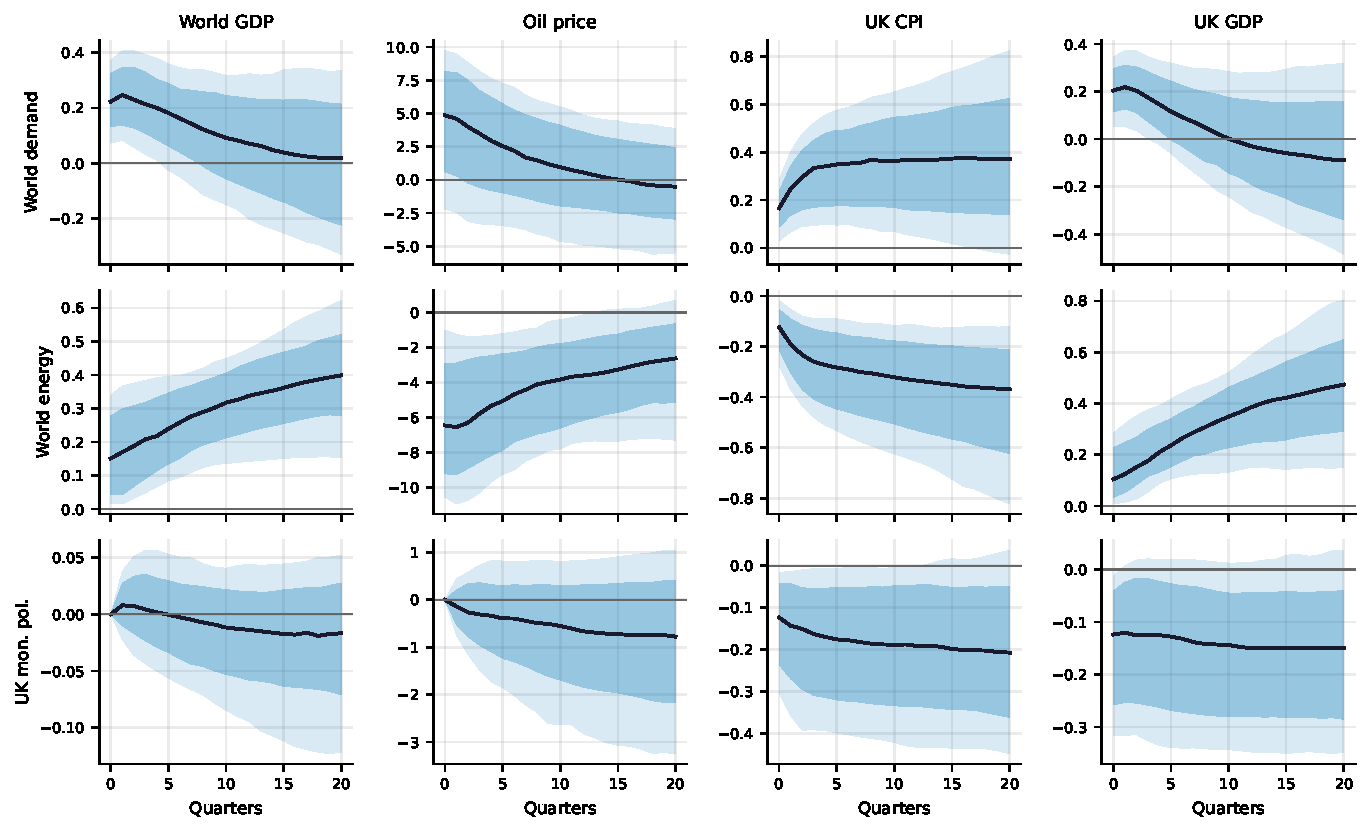
\includegraphics[width=\textwidth]{figures/fig_irf.pdf}
\caption{Impulse responses to one-standard-deviation world demand, world energy and UK monetary policy shocks. Solid line: pointwise posterior median; dark and light bands: 68 and 90 per cent credible bands across accepted draws. Units are $100\cdot\log$ levels (percentage points for Bank Rate). Restrictions are imposed on impact only.}
\label{fig:irf}
\end{figure}

Figure~\ref{fig:fevd} stacks the median FEVD shares for UK GDP and UK CPI by horizon. The pattern that anchors the calibration comparison in Table~\ref{tab:validation} is visible directly: at the one-year horizon the three identified global shocks account for roughly two-fifths of UK GDP variance and roughly half of UK CPI variance, with the world demand share of CPI growing steadily in the horizon. Domestically, UK supply is the largest identified contributor to GDP variance --- and, in this replication's known discrepancy with the paper, also to CPI variance, where the paper attributes more to monetary policy.

\begin{figure}[t]
\centering
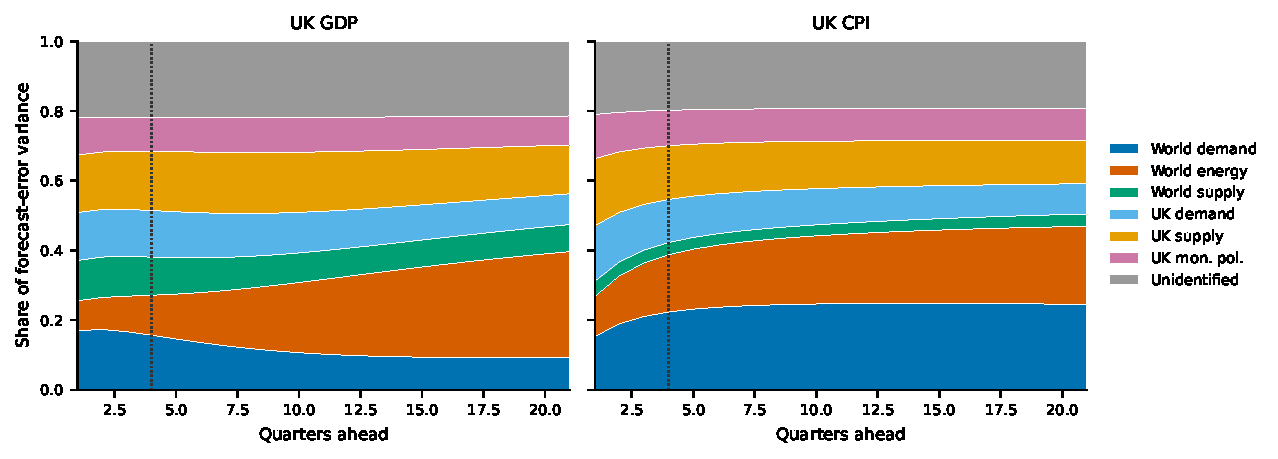
\includegraphics[width=\textwidth]{figures/fig_fevd.pdf}
\caption{Median forecast-error variance decompositions of UK GDP and UK CPI by horizon. The two unidentified shocks are shown combined. Shares are renormalised to sum to one at each horizon after taking pointwise medians.}
\label{fig:fevd}
\end{figure}

Figure~\ref{fig:hd} gives the historical decomposition of year-on-year UK CPI inflation from 2016 --- the model's structural account of the 2021--23 inflation surge and its aftermath. The surge is attributed overwhelmingly to global shocks: contractionary world energy shocks and strong world demand dominate the 2022 bars, with UK-specific shocks and the Covid-dummy component playing supporting roles, and the decomposition unwinding through 2023 as energy shocks reverse. This reproduces the qualitative account in the source paper's Figure~6 and matches the Bank's contemporaneous narrative of imported inflation.

\begin{figure}[t]
\centering
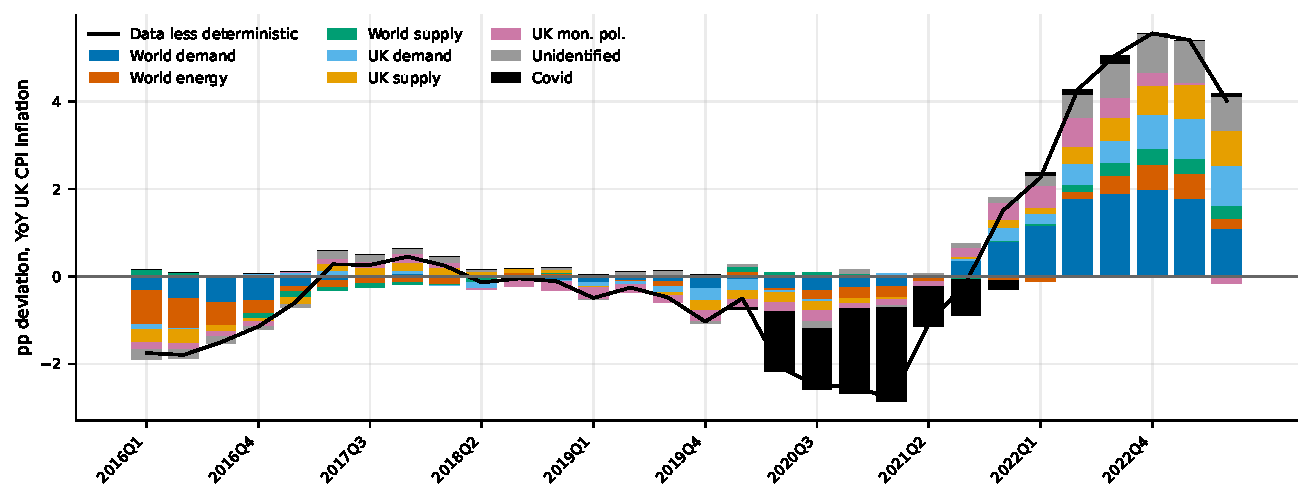
\includegraphics[width=\textwidth]{figures/fig_hd.pdf}
\caption{Historical decomposition of year-on-year UK CPI inflation (deviation from the deterministic component), 2016Q1--2023Q2. Bars: median cumulative contributions of the six identified shocks, the combined unidentified shocks, and the Covid-dummy component; line: data less the deterministic component.}
\label{fig:hd}
\end{figure}

\paragraph{Narrative reproduction.} The estimated shock series reproduce the paper's episodes: the 2008 collapse in world demand, the contractionary world energy shocks of 2022, UK monetary loosening readings after 2022 followed by tightening readings in 2023, and muted shocks during 2020--21 by construction of the Covid dummies. Known caveats are equally documented: median UK GDP responses to world demand and supply shocks decay through zero at long horizons where the paper's remain positive (the paper's path lies inside the replication's bands), and within the global supply side the energy shock contributes more than the non-energy supply shock to world GDP and oil-price variance, where the paper's figure suggests the reverse ordering; the paper's claims about the \emph{combined} supply side are matched.
